% \documentclass{report}
% \setlength{\headheight}{24.1638pt}
% packages
% \usepackage[french]{babel}
% \usepackage[T1]{fontenc}
% \usepackage[utf8]{inputenc}
% \usepackage{mathtools}
% \usepackage{amssymb}
% \usepackage{hyperref}
% \usepackage{float}
% \usepackage{amsthm}
% \usepackage{listings}
% \usepackage{geometry}
% \usepackage{setspace}
% \usepackage{graphicx}
% \usepackage{fancyhdr}
% \usepackage{subcaption}
% \usepackage{cleveref}

% commands
% \newtheorem{defi}{Définition}
% \renewcommand{\thedefi}{\empty{}}

% \renewcommand\headrulewidth{1pt}
% \newcommand{\crule}[3][c]{%
%     \par\noindent
%     \makebox[\linewidth][#1]{\rule{#2\linewidth}{#3}}}
% \renewcommand{\thechapter}{\Roman{chapter}}

% Style de page
% \pagestyle{fancy}
% \fancyhead[L]{}
% \fancyhead[C]{}
% \fancyhead[R]{\leftmark}
% \allowdisplaybreaks
% \geometry{hmargin=3cm,vmargin=2.5cm}


% préambule
% \begin{document}

% \lstset{
%   firstnumber=0, 
%   numbers=left,               
%   frame=single,
%   language=C,                                       
%   showstringspaces=false
% }
\section{Graphiques}
Dans cette section, nous allons conclure sur l'efficacité des deux méthodes, Jacobi et Gauss-Seidel. Pour cela, nous allons d'abord illustrer la différence de performance entre nos deux implémentations.
\subsection{Cas où les méthodes divergent}
Avec les matrices $A_1$ et $A_2$ dans le système à résoudre, nous pouvons remarquer que les méthodes de Jacobi et de Gauss-Seidel divergent. De plus, il est notable que Jacobi diverge beaucoup moins rapidement que Gauss-Seidel.

\begin{figure}[H]
    \centering
    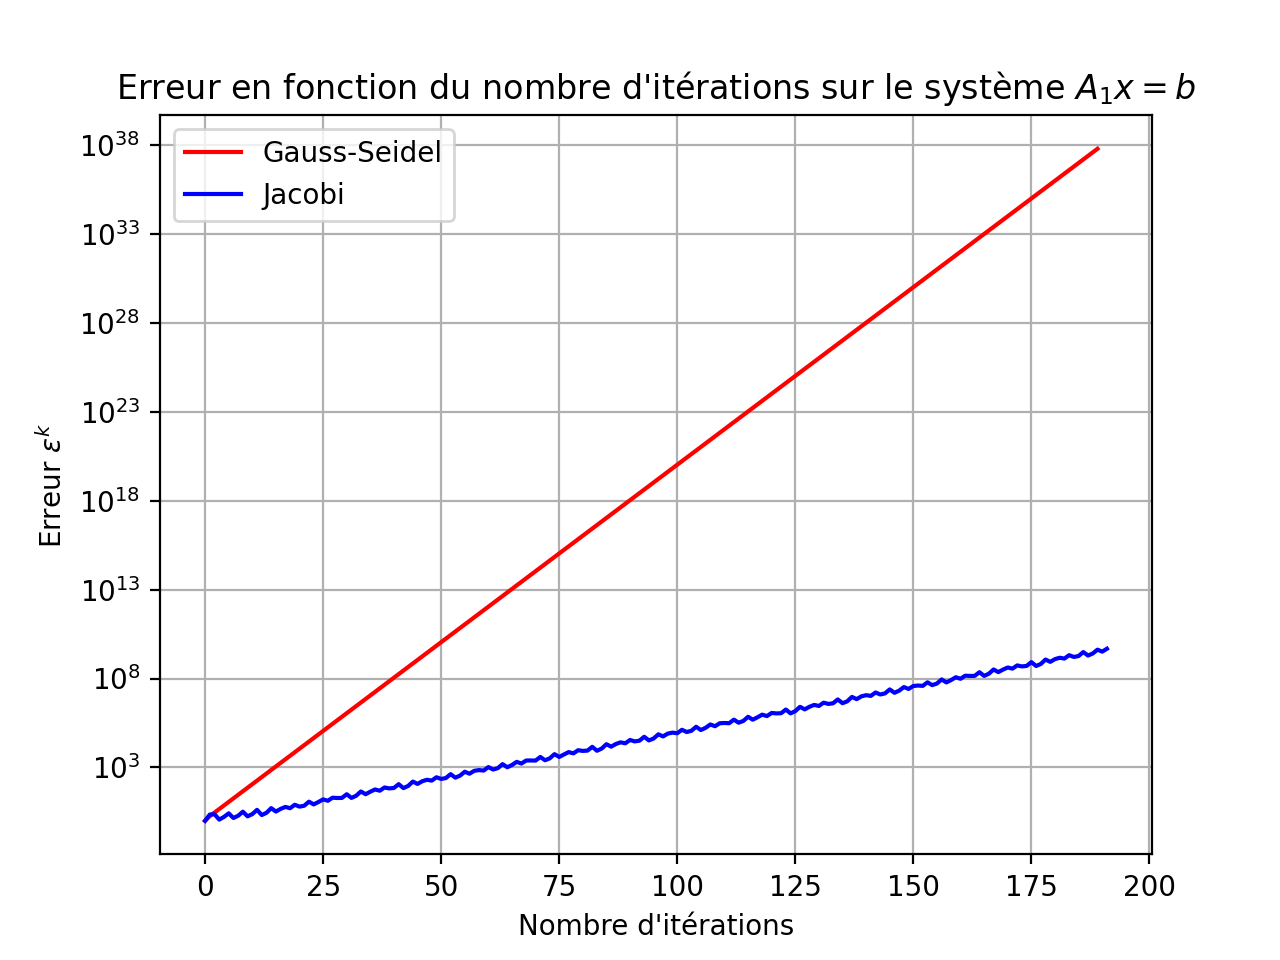
\includegraphics[width=0.75\textwidth]{graphes/graphs/resA1.png}
\end{figure}
\begin{figure}[H]
    \centering
    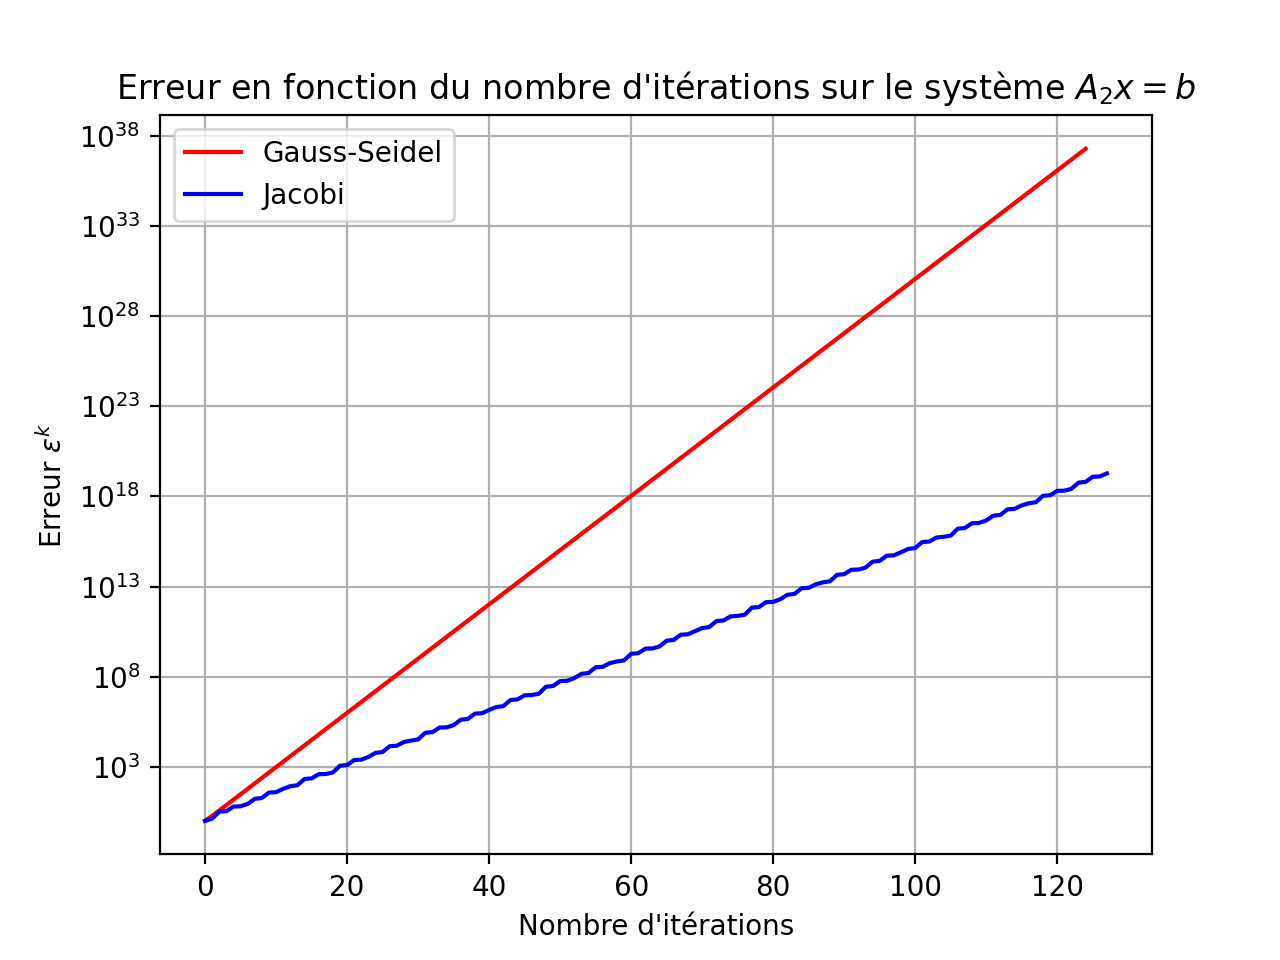
\includegraphics[width=0.75\textwidth]{graphes/graphs/resA2.png}
\end{figure}

\subsection{Cas où les méthodes convergent}
Dans la plupart des cas où la méthode de Jacobi et la méthode de Gauss-Seidel convergent, c'est celle de Gauss-Seidel qui fournit un vecteur solution plus précis et plus rapidement que Jacobi. Autrement dit, l'erreur mesurée dans les algorithmes décroit plus rapidement au fil des itérations dans la méthode de Gauss-Seidel.
Voici quelques graphiques pour illustrer ces cas.
\begin{figure}[H]
    \centering
    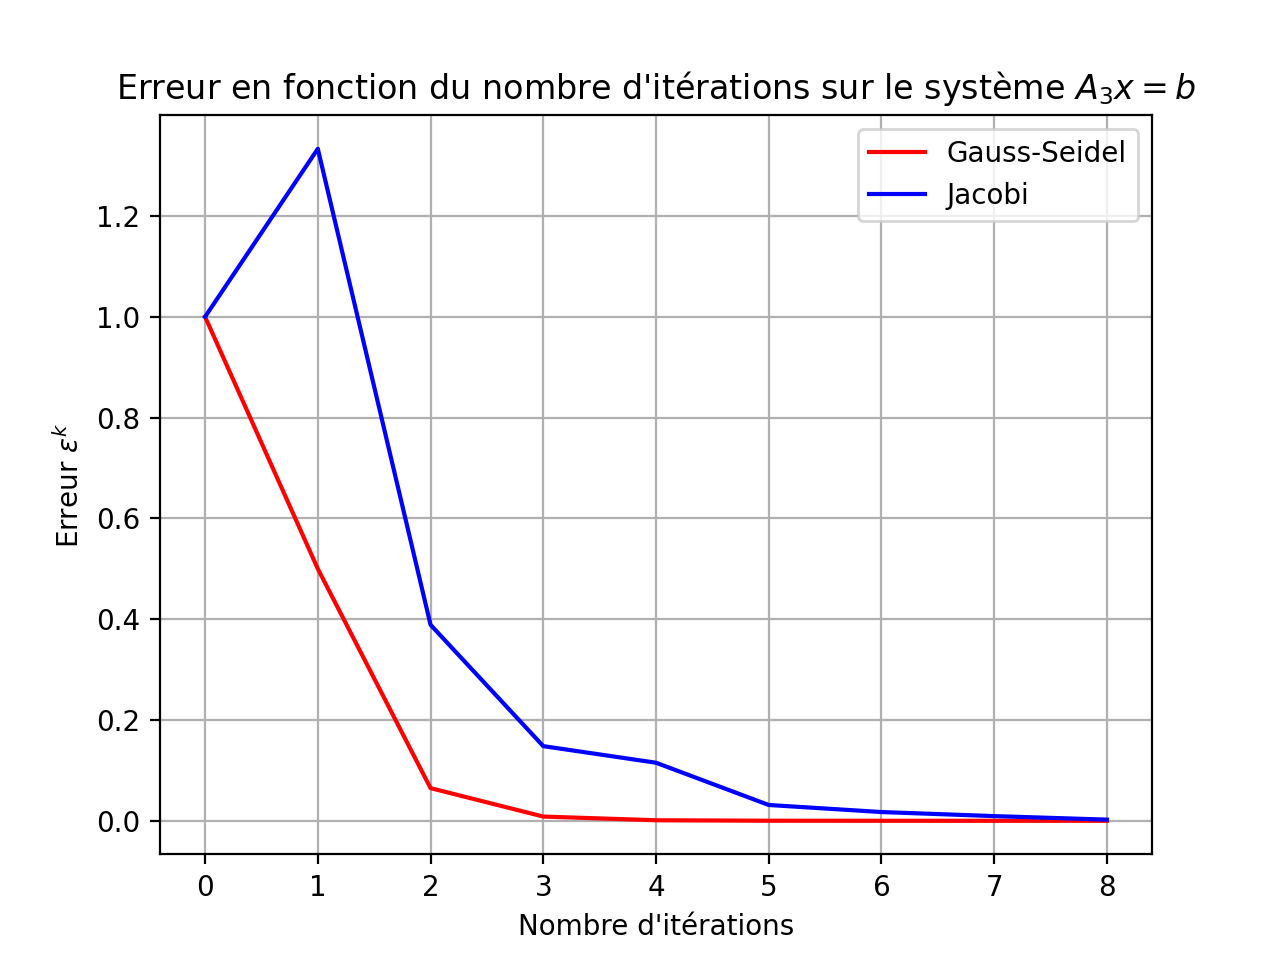
\includegraphics[width=0.75\textwidth]{graphes/graphs/resA3.png}
\end{figure}
\begin{figure}[H]
    \centering
    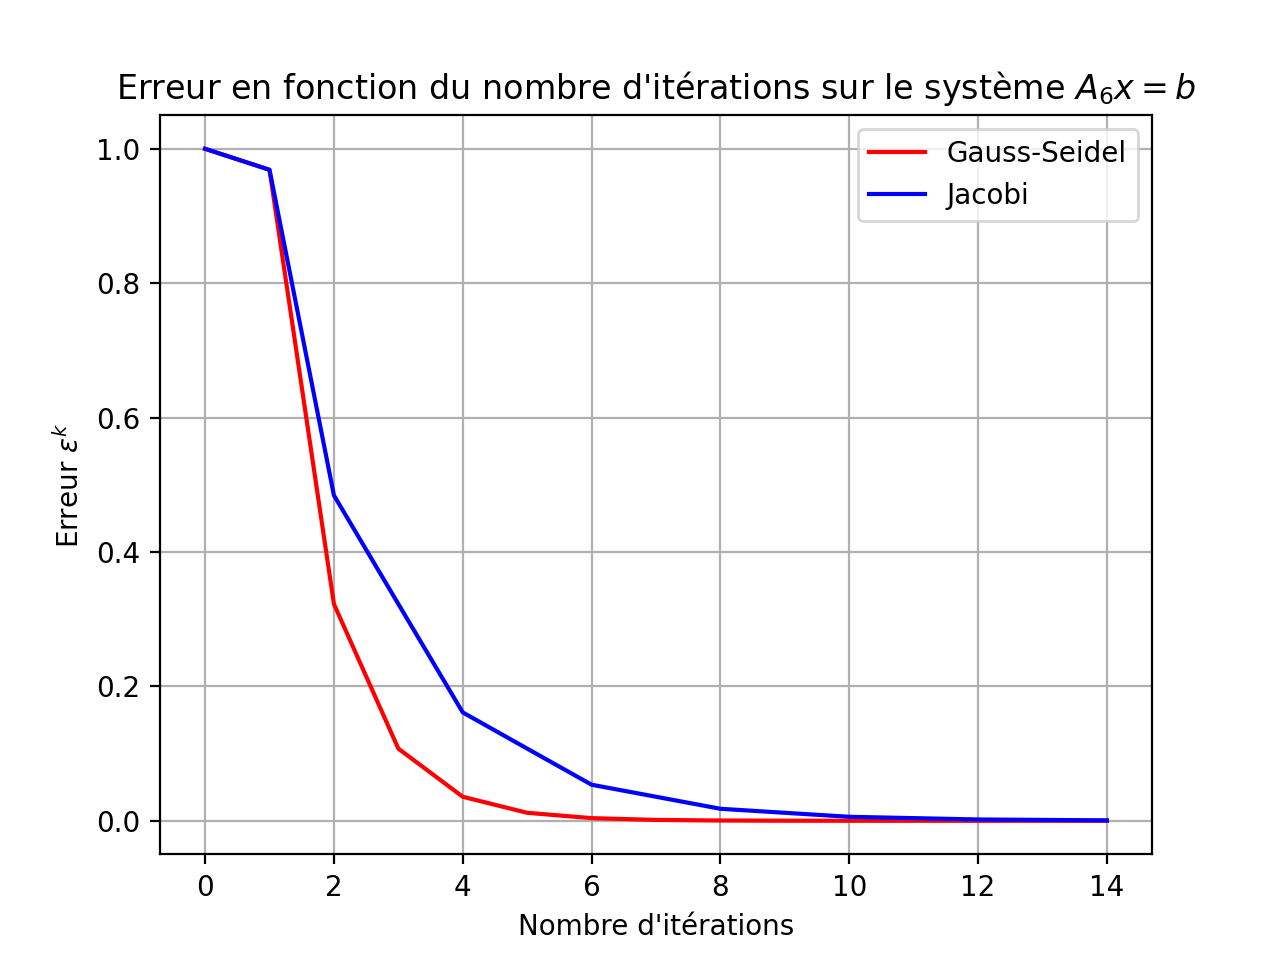
\includegraphics[width=0.75\textwidth]{graphes/graphs/resA6.png}
\end{figure}
\begin{figure}[H]
    \centering
    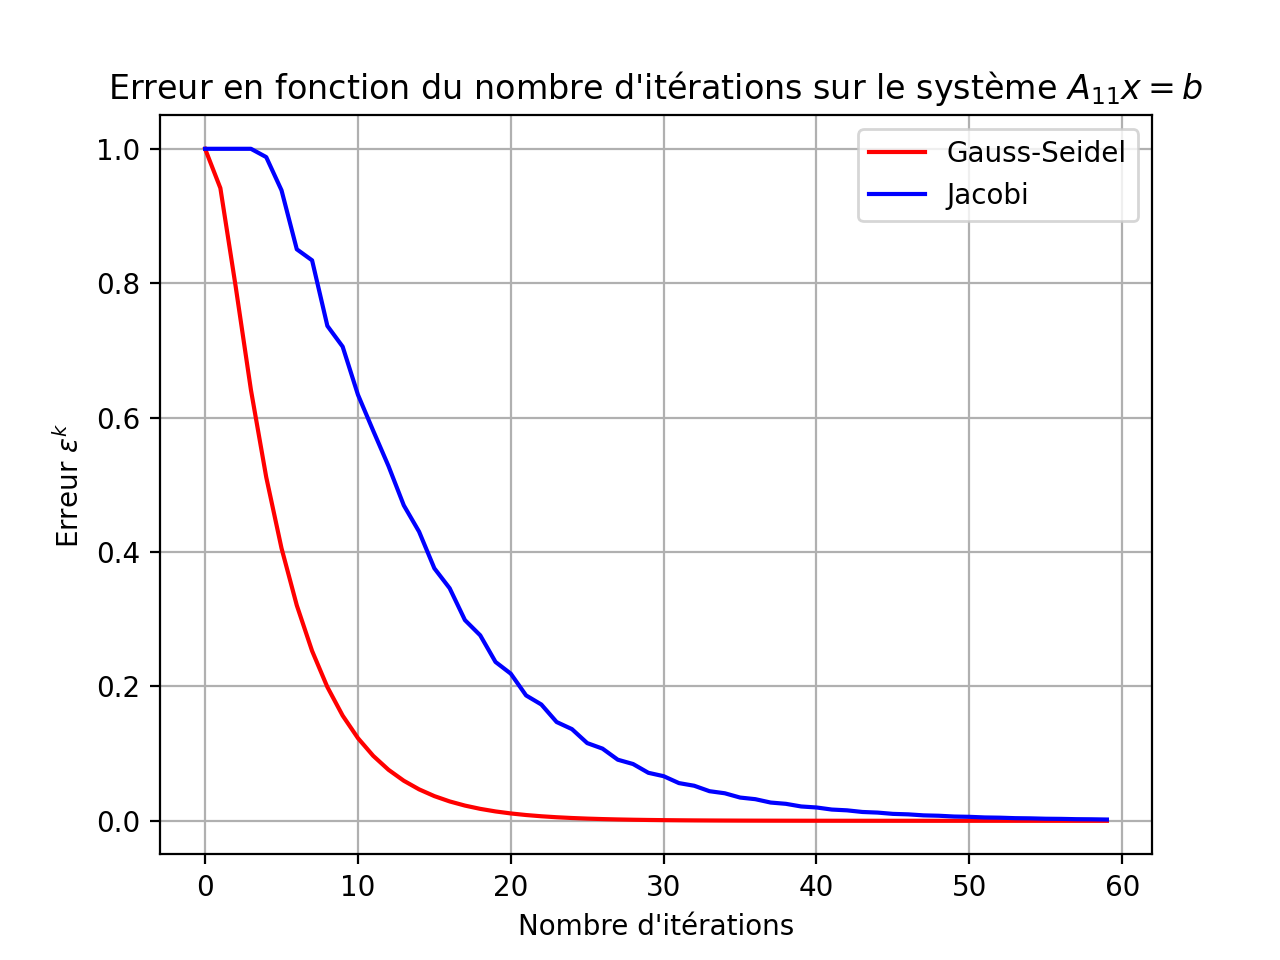
\includegraphics[width=0.75\textwidth]{graphes/graphs/resA11.png}
\end{figure}
Il y a quelquefois certains cas où Jacobi converge plus vite que Gauss-Seidel. C'est le cas avec le système composé avec la matrice $A_4$.
En voici la preuve graphique:
\begin{figure}[H]
    \centering
    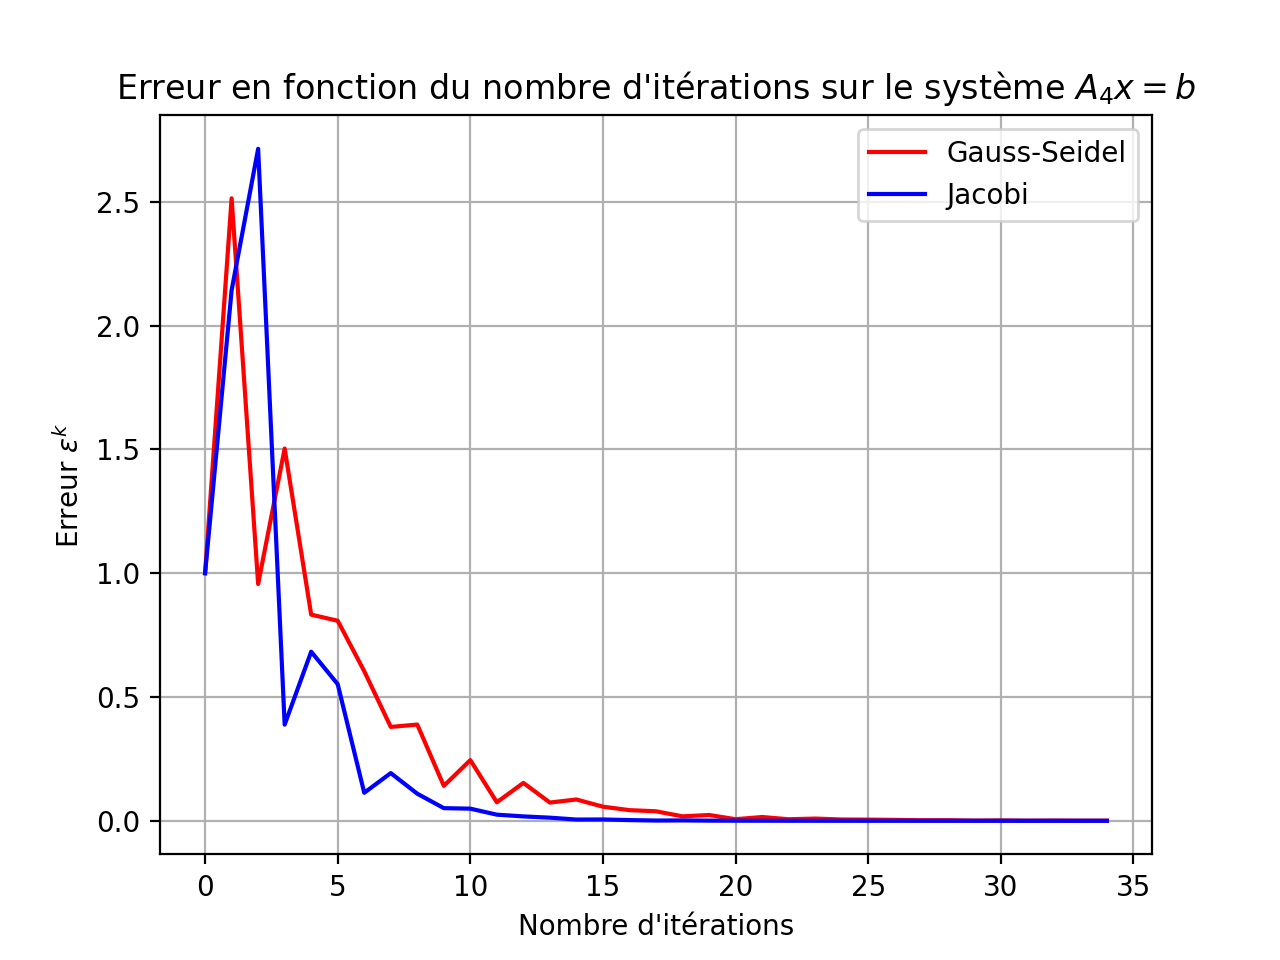
\includegraphics[width=0.75\textwidth]{graphes/graphs/resA4.png}
\end{figure}

Enfin, voici la représentation graphique qui illustre de manière plus condensée les propositions ci-dessus sur toutes les matrices du TP (lorsque la résolution converge).
\begin{figure}[H]
    \centering
    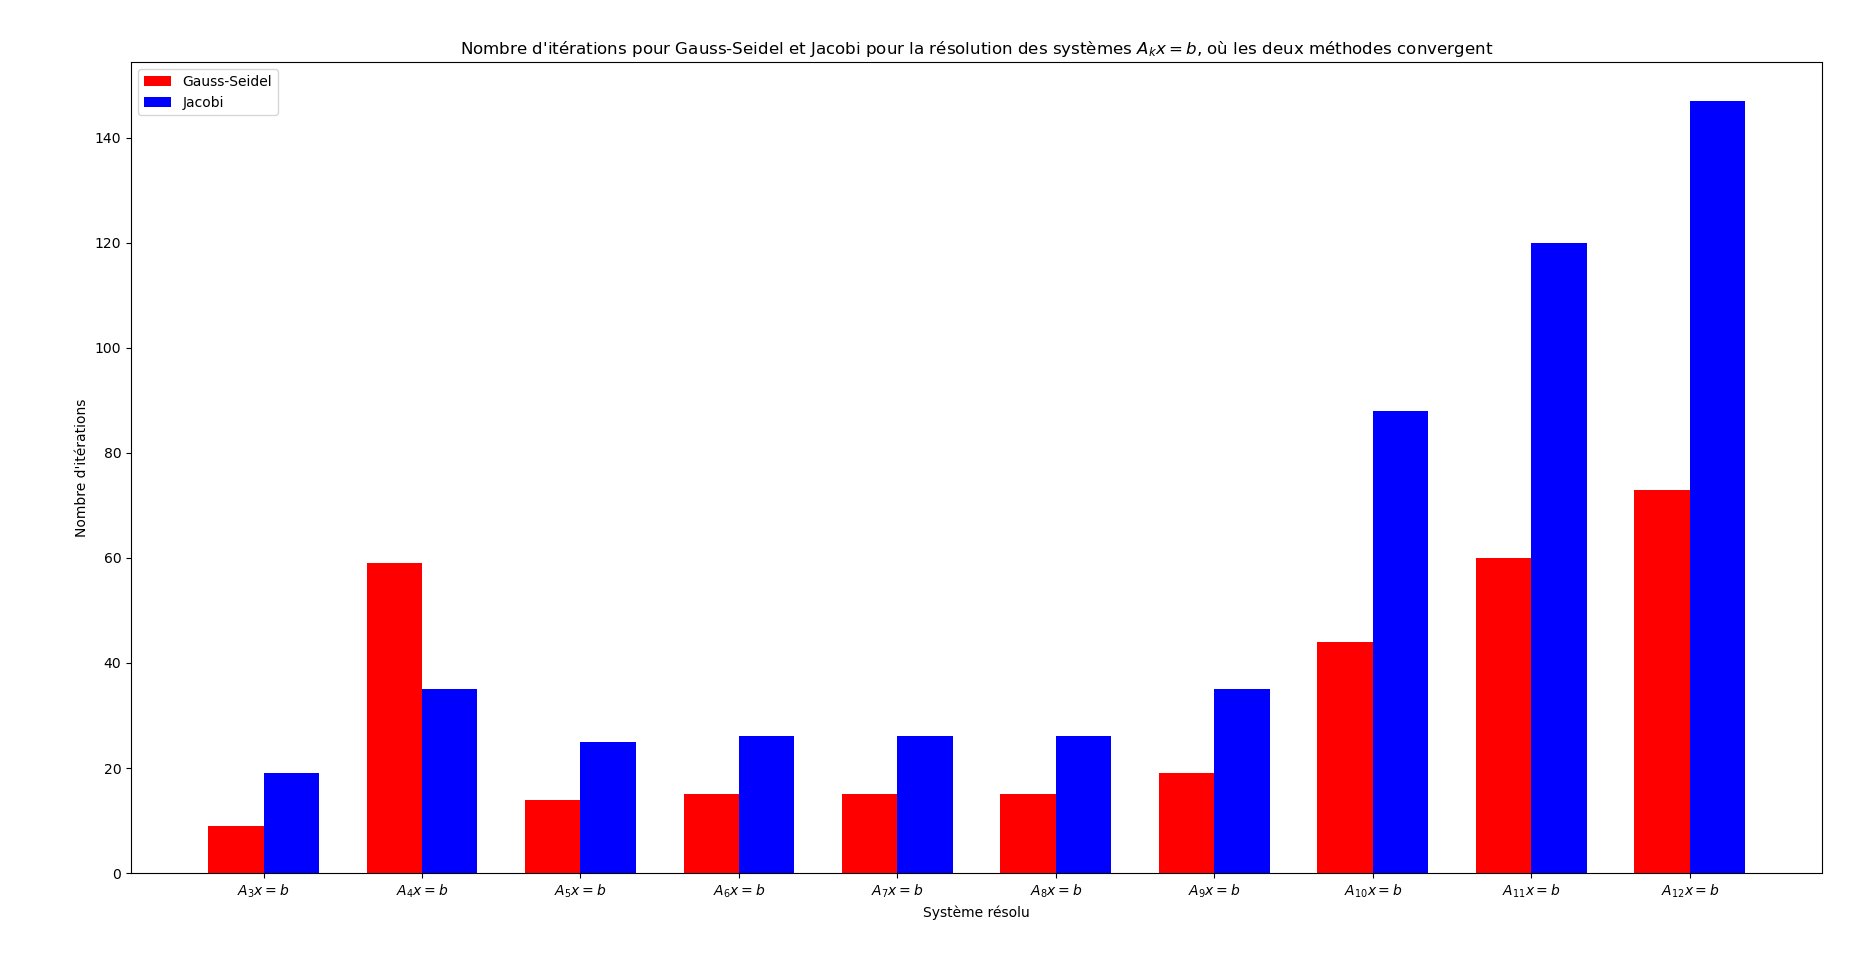
\includegraphics[angle=90, width=0.8\textwidth]{graphes/graphs/baton.png}
\end{figure}
% \end{document}

